\subsection{Modelo Conceptual}

\begin{figure}
  \begin{center}
	%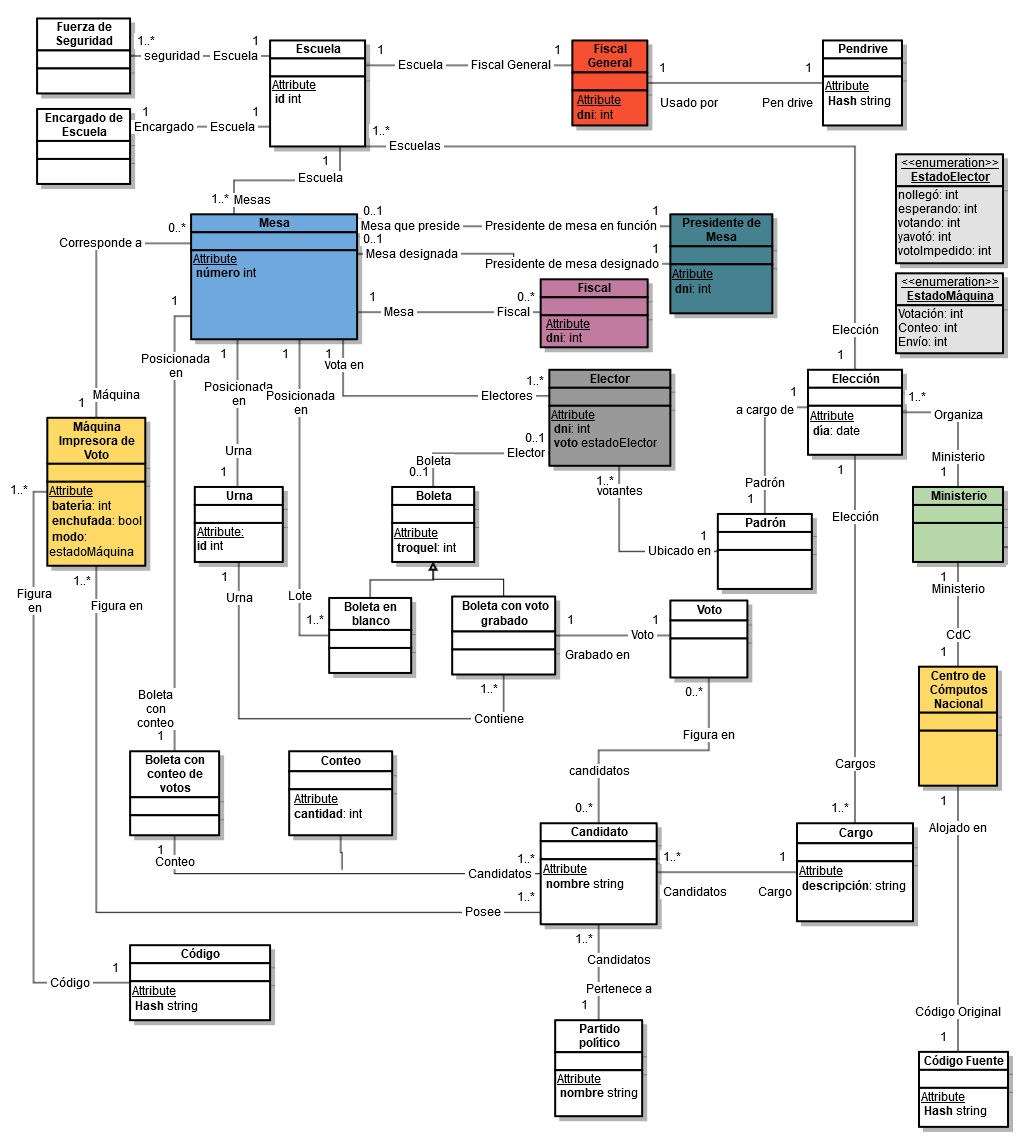
\includegraphics[scale=0.64]{imagenes/clases.png}
  \end{center}
\end{figure}

\newpage
\subsubsection{OCL}


\subsubsection*{Mesa}

\textit{context Mesa
inv}
\begin{enumerate}

\item \textbf{Los n\'umeros de las mesas son únicos.}

$Mesa.AllInstances \rightarrow forAll(m_1, m_2 | m_1.numero <> m_2.numero))$

\item  \textbf{No hay dos mesas con el mismo fiscal.}

$Mesa.AllInstances \rightarrow forAll(m_1, m_2 | m_1.Fiscal.dni <> m_2.Fiscal.dni))$

\item \textbf{No hay dos mesas con electores en común.}

$Mesa.AllInstances \rightarrow \\
 forAll(m_1, m_2 | m_1.Electores \rightarrow \\
 forAll(e_1 | m_2.Electores \rightarrow Select(e_2 | e_1.dni==e_2.dni) \rightarrow Size() == 0))$

\item \textbf{No hay dos mesas con el mismo presidente de mesa.}

$Mesa.AllInstances \rightarrow \\
forAll(m_1, m_2 | m_1.PresidenteDeMesaDesignado.dni <> m_2.PresidenteDeMesaDesignado.dni))$

\item \textbf{Los presidentes de mesa votan en la misma mesa que son presidentes.}

$self.Electores \rightarrow Exists(e | self.PresidenteDeMesaDesignado.dni == e.dni)$

\item \textbf{La cantidad de Boletas Sin voto grabado y con voto grabado de la mesa debe ser mayor o igual a la cantidad de electores de dicha mesa.}

$self.Lote \rightarrow Size() + self.Urna.Contiene \rightarrow Size () \geq self.Electores \rightarrow Size()$

\item \textbf{La cantidad de Boletas Con voto grabado de la mesa debe ser menor o igual a la cantidad de electores de dicha mesa.}

$self.Urna.Contiene  \rightarrow  Size() \leq self.Electores \rightarrow Size()$

\item \textbf{Si la máquina está en modo votación es porque s\'olo un elector, o ninguno, está votando (No puede haber dos electores por mesa votando a la vez).}

$self.Maquina.modo == votacion$  IMPLIES  $ \\
self.Electores \rightarrow select(e | e.voto == votando) \rightarrow Size() \leq 1$

\item \textbf{Si la máquina está en modo conteo es porque no hay ningún elector de la mesa votando o esperando para votar.}

$self.Maquina.modo == votacion$  IMPLIES  $ \\
self.Electores \rightarrow \\
select(e | e.voto == votando$ OR $e.voto == esperando) \rightarrow Size() = 0$

\item \textbf{La máquina de la mesa puede estar en modo votación o conteo pero no en envio.}

$self.Maquina.modo <> envio$

\item \textbf{No puede haber un fiscal y un presidente de mesa con el mismo dni.}

$self.Fiscales \rightarrow \\
select(f | f.dni == self.PresidenteDeMesaEnFuncion.dni OR \\
f.dni == self.PresidenteDeMesaDesignado.dni) \rightarrow \\
Size() == 0 $

\item \textbf{Todos los candidatos de la elecci\'on est\'an en la boleta de conteo de votos (incluyendo cuando la cantidad de votos recibida por el candidato en esa mesa fuese 0).}

$self.Escuela.Eleccion.Cargos \rightarrow \\
forAll(car | car.Candidatos \rightarrow \\
forAll(can_1 | self.BoletaConConteo.Candidatos \rightarrow \\
Exists(can_2| can_1.nombre == can_2.nombre $ AND $car.descripcion==can_2.cargo.descripcion)))$

\end{enumerate}

\subsubsection*{Boleta}

\textit{context Boleta
inv}

\begin{enumerate}

\item \textbf{Los id de las boletas son únicos.}

$Boleta.AllInstances() \rightarrow forAll(b_1, b_2 | b_1.troquel <> b_2.troquel)$

\item \textbf{La boleta con voto grabado tiene elector.}

$self.IsKindOf?(BoletaConVotoGrabado)$  IMPLIES  $self.Elector \rightarrow Size() == 1 $

\item \textbf{Si un elector tiene una boleta en blanco, entonces esta boleta está en la mesa que el elector vota.}

$self.IsKindOf(BoletaEnBlanco)?$ AND $self.Elector \rightarrow Size() == 1 $ IMPLIES $\\
self.PosicionadaEn.numero == self.Elector.VotaEn.numero$

\item \textbf{Si un elector tiene una boleta con voto grabado, entonces esta boleta está en la urna que el elector vot\'o.}

$self.IsKindOf(BoletaConVotoGrabado)? $  IMPLIES  $\\
self.Urna.PosicionadaEn.numero == self.Elector.VotaEn.numero$

\item \textcolor{red}{Los votos de las boletas son de candidatos de la eleccion q vota el elector. Aclarar en el informe que esto hace q los votos contabilizados en la boleta de conteo tambien son de la misma eleccion ya q las boletas entre si son consistentes y no hace falta aclararlo extra por ocl}

\end{enumerate}

\subsubsection*{Boleta con Conteo de Votos}

\textit{context Boleta con Conteo de Votos
inv}

\begin{enumerate}
\item \textbf{La boleta con Conteo de votos no tiene candidatos repetidos.}

$self.Candidatos \rightarrow forAll(c_1, c_2| c_1.nombre <> c_2.nombre)$

\end{enumerate}
\subsubsection*{Conteo}

\textit{context Conteo
inv}

\begin{enumerate}

\item \textbf{La boleta con conteo tiene la cantidad de votos que recibi\'o cada candidato en esa mesa.}

$self.Cantidad == \\
self.BoletaConConteodeVotos.mesa.boletaConVotoGrabado \rightarrow \\
select(b | b.voto.candidato  \rightarrow exist(c | c==self.candidato)) \rightarrow size() $

\end{enumerate}

\subsubsection*{Voto}

\textit{context Voto
inv}

\begin{enumerate}
\item \textbf{No tiene dos candidatos con el mismo cargo.}

$self.Candidatos  \rightarrow forAll(c_1, c_2 | )$

\item \textbf{No tiene dos candidatos con el mismo nombre.}
\end{enumerate}

\subsubsection*{Urna}

\textit{context Urna
inv}

\begin{enumerate}
\item \textbf{Las boletas con voto grabado de la urna son sólo de votantes de la mesa que figura la urna.}
\item \textbf{En una misma urna no hay dos boletas con el mismo elector.}    
\item \textbf{Los id de las urnas son únicos.}
\end{enumerate}

\subsubsection*{Escuela}

\textit{context Escuela
inv}

\begin{enumerate}
\item \textbf{Los id de las mesas son únicos.}
\item \textbf{No puede haber un fiscal general y un fiscal con el mismo dni.}
\item \textbf{No puede haber un fiscal general y un presidente de mesa con el mismo dni.}
\end{enumerate}

\subsubsection*{M\'aquina Impresora de Voto}

\textit{context M\'aquina Impresora de Voto
inv}

\begin{enumerate}
\item \textbf{Los candidatos de todas las máquinas son los mismos.}

\end{enumerate}

\subsubsection*{Elector}

\textit{context Elector
inv}

\begin{enumerate}
\item \textbf{Los dni de los electores son únicos.}
\item \textbf{El elector puede no tener ninguna boleta, tener una vacía o tener una con voto.}
\item \textbf{No puede haber un elector y una persona que no figura en el padrón con el mismo dni.}
\item \textbf{Si el elector no llegó, está esperando o no lo dejaron votar no tiene boleta.}
\item \textbf{Si el elector está votando tiene una boleta en blanco.}
\item \textbf{Si el elector ya votó tiene una boleta con voto grabado.}
\end{enumerate}

\subsubsection*{Partido Pol\'itico}

\textit{context Partido Pol\'itico
inv}

\begin{enumerate}
\item \textbf{No hay dos partidos políticos con ningún candidato en común.}
\end{enumerate}

\subsubsection*{Centro de C\'omputos}

\textit{context Centro de C\'omputos
inv}

\begin{enumerate}
\item \textbf{Hay uno solo.}
\end{enumerate}

\subsubsection*{C\'odigo}

\textit{context C\'odigo
inv}

\begin{enumerate}
\item \textbf{El hash del código es el mismo del hash del código fuente. }  
\item \textbf{El hash del código es el mismo del hash de todos los pendrives de los fiscales.}   
\end{enumerate}  

\subsubsection*{Ministerio}

\textit{context Ministerio
inv}

\begin{enumerate}
\item \textbf{Hay un solo ministerio.}
\end{enumerate}

\subsubsection*{Presidente de Mesa}

\textit{context Presidente de Mesa
inv}

\begin{enumerate}
\item \textbf{Si el presidente de mesa del ministerio está presente, no hay presidente ad hoc.}
\item \textbf{Si la mesa tiene un solo presidente de mesa, tiene que ser el de Ministerio.}
\item \textbf{Si hay dos presidentes, el del ministerio debe estar ausente.}
\item \textbf{Si alguien voto, debe haber votado el presidente mesa antes (El Ad hoc si la mesa tiene dos presidentes, o el del ministerio si tiene uno solo).}
\end{enumerate}

\subsubsection*{Candidato}

\textit{context Candidato
inv}

\begin{enumerate}
\item \textbf{Los id de los candidatos son únicos.}
\end{enumerate}
